%\begin{figure}[h]
%	\centering\includegraphics[width=0.8\textwidth]{fig/figure_4}
%	\caption{Extrem coole Grafik!}
%\end{figure}


% SUBFIGURE
%\begin{figure}[h]
%	\centering
%	\subfigure[]{\includegraphics[width=0.49\textwidth]{fig/2_a_plot}}
%	\subfigure[]{\includegraphics[width=0.49\textwidth]{fig/2_b_plot}}
%	\caption{\textbf{a)} Temperatur des Aluminium Hohlzylinders gegen die Zeit aufgetragen, \textbf{b)} Änderung der Temperatur gegenüber der Temperatur aufgetragen. Jeweils unter Verwendung des Heizdrahtes.}
%	\label{fig:2_1_plot}
%\end{figure}

\section{Dispersionsrelation}
\subsection{Einatomige Kette}

Über die Messwerte des Versuchs wird gemittelt um die Dispersionsrelation der einatomigen Kette zu bestimmen. Die Werte für die Wellenvektoren wurden dabei mit Hilfe der Formel aus der Vorbereitungshilfe und der gemessenen Länge des Versuchsaufbaus berechnet:
\begin{align}
	L &= 13a_1\\
	k_{\textrm{n}} &= \frac{n\pi}{13a_1}
\end{align}
Die Länge wurde gemessen als
\begin{equation}
	L = 5,43 \pm\; 0,01\;\si{\meter}
\end{equation}
Die Dispersionsrelation mit den gemittelten Messwerten ist in Abbildung \ref{fig:a1_one} dargestellt.
\begin{figure}[h]
	\centering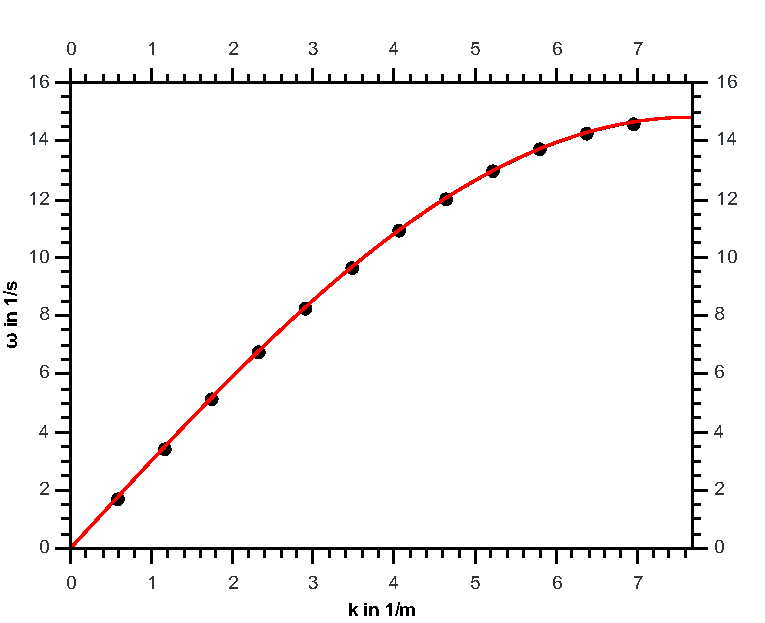
\includegraphics[width=0.8\textwidth]{fig/a1_one}
	\caption{Dispersionsrelation der einatomigen Kette (1. Brillouinzone)}
	\label{fig:a1_one}
\end{figure}
Die Regression an die Messwerte ergibt für die Gitterkonstante
\begin{equation}
	a_1 = (0,409 \pm 0,001)\;\si{\meter}
\end{equation}
und damit für den Rand der 1. Brillouinzone
\begin{equation}
	k_{\textrm{max}} = \frac{\pi}{a_1} = (7,68 \pm 0,02)\;\si{\per\meter}
\end{equation}
Der Fehler ergibt sich über die Gaußsche Fehlerfortpflanzung.
Die Abweichung des so bestimmten Werts für die Gitterkonstante $a_1$ weicht nur um ca. 2\;\% vom erwarteten theoretischen Wert von $a_1 = \frac{L}{13}$ ab.
%c = 14,64 pm 0,02

\subsection{Zweiatomige Kette}

Laut Vorbereitungshilfe beträgt der theoretische Wert der Wellenvektoren für die zweiatomige Kette
\begin{equation}
	 k_{\textrm{n}} = \frac{n\pi}{6,5a_2}
\end{equation}
Wobei die Gitterkonstante $a_2$ berechnet werden kann mit
\begin{equation}
	a_2 = \frac{L}{6,5} = (0,835 \pm 0,0015)\;\si{\meter}
\end{equation}
Somit beträgt der theoretische Rand der 1. Brillouinzone
\begin{equation}
	k_{\textrm{max}} = \frac{\pi}{a_2} = (3,762 \pm 0,007)\;\si{\per\meter}
\end{equation}
Die gemittelten Messwerte sind in Abbildung \ref{fig:a1_two} dargestellt.
\begin{figure}[h]
	\centering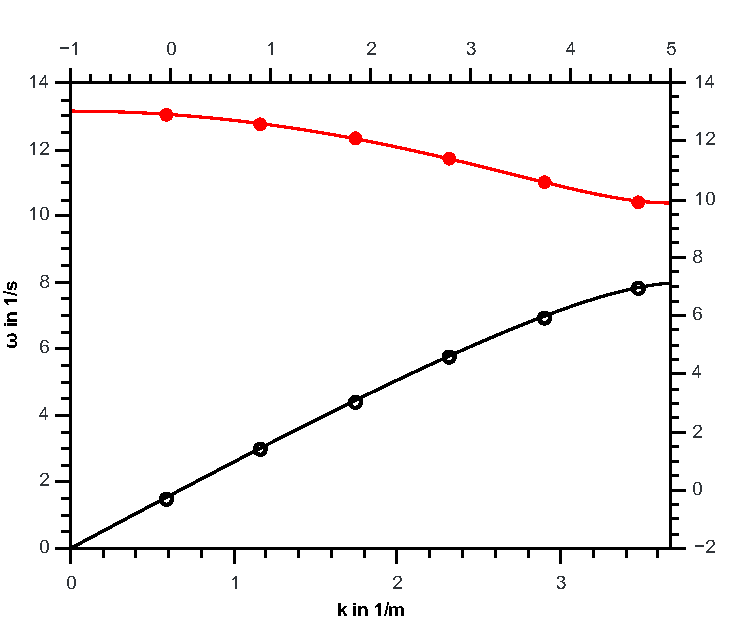
\includegraphics[width=0.8\textwidth]{fig/a1_two}
	\caption{Dispersionsrelation der zweiatomigen Kette (1. Brillouinzone)}
	\label{fig:a1_two}
\end{figure}
Die roten Datenpunkte stellen den optischen Zweig da, die hohlen schwarzen Datenpunkte den akustischen Zweig.

\section{Schallgeschwindigkeit}

Die Schallgeschwindigkeit lässt sich aufgrund der Kleinwinkelnäherung aus einer linearen Regression zwischen dem Ursprung und dem ersten Wertepaar bestimmen.\\
Dies ergibt für die beiden unterschiedlichen Ketten:
\begin{itemize}
	\item Einatomige Kette: $v_{schall,1} = \frac{\omega_1}{k_1} = (3,007 \pm 0,0055)\;\si{\meter\per\second}$\\
	\item Zweiatomige Kette: $v_{schall,2} = $
\end{itemize}
Die Fehler sind dabei rein systematisch mit Gaußscher Fehlerfortpflanzung berechnet, da nicht genügend Messwerte verwendet werden um einen statistischen Fehler zu erhalten. Es wurde ein systematischer Fehler auf die Frequenz von $\Delta\omega = 0,001 \si{\per\second}$ angenommen.

\section{Massenverhältnis}

Das Massenverhältnis der beiden unterschiedlichen Gleiter ist gegeben durch
\begin{equation}
	\frac{M}{m} = 2\cdot\frac{v_{schall,1}}{v_{schall,2}} - 1 = 
\end{equation}

\section{Bestimmung der Federkonstanten}
\subsection{Aus der Dispersionsrelation der einatomigen Kette}

Stellt man die Dispersionsrelation der einatomigen Kette um, erhält man eine Formel zur Bestimmung der Federkonstanten
\begin{equation}
	D = \frac{m\omega^2}{4\sin{\frac{ka_1}{2}^2}}
\end{equation}
Nach Bestimmung der Federkonstanten für jedes Wertepaar und anschließende Mittelung ergibt sich ein Wert von
\begin{equation}
	D = 27,615\;\si{\kilogram\per\square\second}
\end{equation}\\
Alternativ lässt sich die Federkonstante aus der Regression der Dispersionsrelation der einatomigen Kette bestimmen.
Die Regression ergab als Vorfaktor für den Sinus $C = 14,64 \pm 0,02$. Damit lässt sich die Federkonstante bestimmen als
\begin{equation}
	D = (27,01 \pm 0,07)\;\si{\kilogram\per\square\second}
\end{equation}

\subsection{Aus der Schallgeschwindigkeit der einatomigen Kette}

Mit der bereits berechneten Schallgeschwindigkeit folgt:
\begin{equation}
	D = m\cdot\left(\frac{v_{schall,1}}{a_1}\right)^2 = (27,2 \pm 0,16)\;\si{\kilogram\per\square\second}
\end{equation}

\section{Amplitudenverhältnisse}



\begin{figure}[h]
	\centering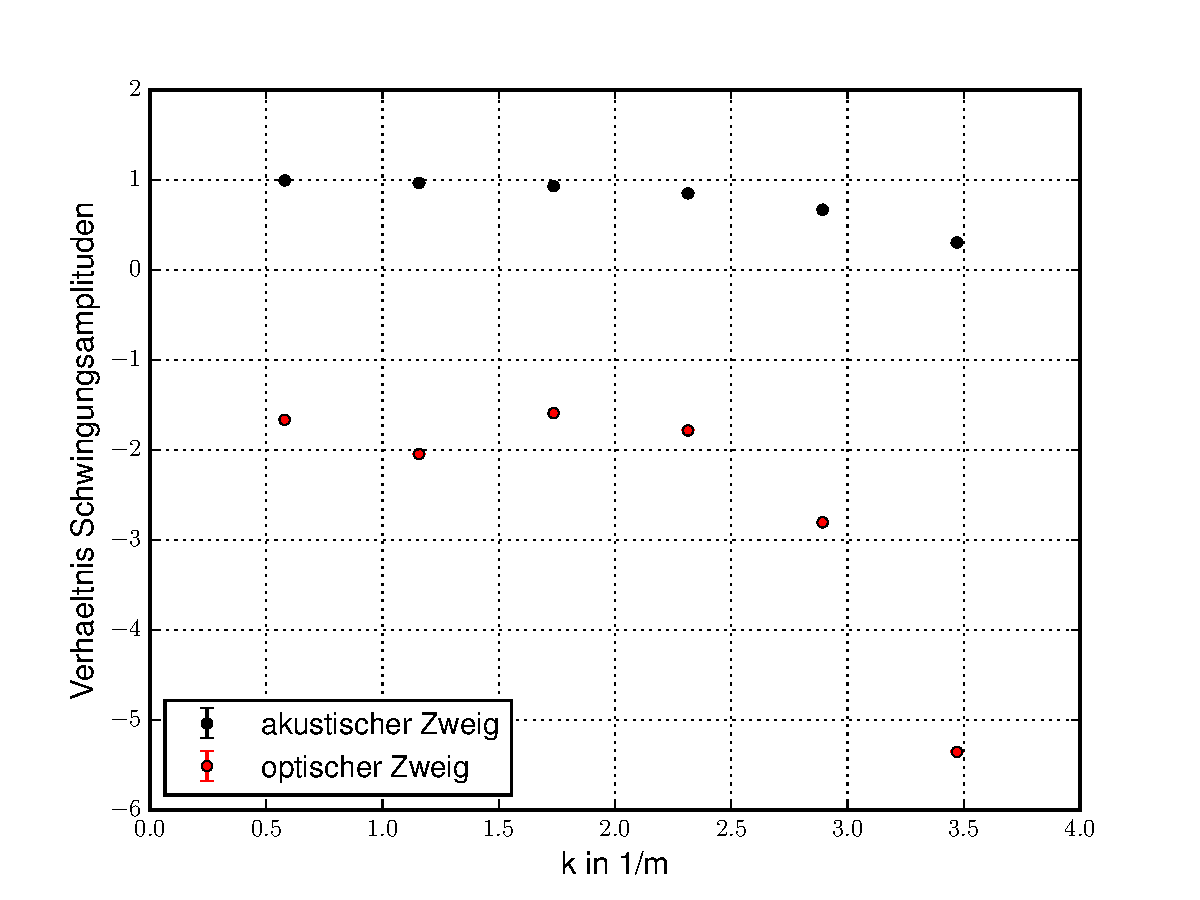
\includegraphics[width=0.8\textwidth]{fig/amplituden}
	\caption{Amplitudenverhältnisse der beiden Zweige.}
	\label{fig:amplituden}
\end{figure}